\section{Descripci\'on de la Soluci\'on}

\subsection{Simulated annealing}
\subsubsection{Definición}
Simulated annealing (Recocido Simulado en español), respecto a las ciencias de la computación, es una metaheuristica para problemas de optimización global, aplicandose a la heurística de Búsqueda Local Aleatoria. La técnica fue presentada por Kirkpatrick, Gelatt y Vecci (1982) y ha sido
muy empleado para resolver problemas combinatorios.
La idea surge del proceso físico conocido como
recocido en el cual, se eleva la temperatura de un
sólido hasta el punto que se vuelve líquido, a continuación
la temperatura se disminuye de forma paulatina
para obtener una estructura cristalina sin defectos
y que puede considerarse como un estado de
mínima energía. Cada descenso de temperatura debe
ser lo suficientemente pequeño para que el sistema
no adquiera una estructura cristalina con defectos,
además el sistema debe permanecer un tiempo
suficiente a una misma temperatura para permitir
alcanzar un estado estacionario, en otras palabras,
que las partículas vuelvan a reacomodarse.


Se parte de una solución inicial posible $S_{i}$, luego se selecciona
una solución posible $S_{j}$ dentro de una vecindad, enseguida
se evalúa la calidad de la solución posible
empleando una función de costo f(x) asociada a cada posible solución S del problema.\\

Si la nueva solución posible $S_{j}$ es mejor que la actual
(de acuerdo al costo), se acepta, de lo contrario
se selecciona de acuerdo a una probabilidad, para
Simulated annealing dicha probabilidad de selección
está dada por la ecuación (1) que se conoce como
el criterio de Metropolis; a $temp$ se le conoce como
el parámetro de control; este valor se inicia con un valor
suficientemente grande para que cualquier solución
tenga una probabilidad alta de ser seleccionada,
a medida que $temp$ disminuye, la probabilidad de
aceptar soluciones factibles de mala calidad disminuye. El enfriamiento
se realiza empleando el sistema geométrico
dado por la ecuación (2), donde $\alpha$ es un parámetro
fijo.

\begin{equation*}
\begin{array}{ll@{}ll}
criterio(S_{i}, S_{j})= exp( (costo(S_{i}) - costo(S_{j})) / temp) & (1) 
\end{array}
\end{equation*}

\begin{equation*}
\begin{array}{ll@{}ll}
temp_{k+1} =  temp_{k} *  \alpha & (2)
\end{array}
\end{equation*}


\subsubsection{Implementación para resolver Sudoku}
Antes de ir directo al algoritmo hay que tener en cuenta las diferentes elecciones que hicimos para encontrar una solución inicial, mejorarla y  decidir cuando una solución es mejor que otra.
\paragraph{Solución inicial} 
Como el algoritmo así lo requiere, debemos partir de una solución inicial para intentar mejorarla y en el mejor de los casos poder resolverla. Una primera opción que se puede pensar es, a partir de las celdas iniciales, rellenar todas las celdas vacías con valores aleatorios directamente. Sin descartar totalmente esta idea fuimos un poco más allá. Básicamente intentamos resolver el Sudoku lo más que podamos, estando siempre seguro de que los valores que pongamos en las celdas son los correctos. Para esto analizamos los posibles valores que pueden ir en cada celda, eliminando de esas posibilidades valores que estén en la misma fila, columna o caja. Luego de esto, en caso de detectar que una celda tiene un solo valor posible, se rellenará la celda con ese valor y se lo considerará correcto ya que fue deducido de la configuración inicial. En caso de que no haya valores posibles para esa celda, indicará que esa configuración inicial no tiene solución posible. Por cada celda que se rellene se deberá recalcular todo el proceso de nuevo, hasta que en algún ciclo no haya modificaciones. \\Una vez que se terminó de deducir lo máximo posible será el momento de rellenar las celdas que quedaron vacias. Para este punto intentaremos ser lo menos aleatorio posible, y para tal caso seleccionaremos entre los posibles valores que pueden tener la celda, que ya habíamos calculado en el punto anterior. Y en caso de que para una celda ya no haya posibles valores, es el momento en que se le asignará uno aleatorio, siempre respetando la formulación (3) que se menciona en la sección anterior, es decir, se respetará en todo momento que no haya celdas inválidas en las cajas.
\paragraph{Función de costo}
El costo (o penalización) va a depender de la cantidad de celdas "ilegales" que tenga la cuadricula. Es decir, cuando haya una celda que se repita en la fila, columna o caja se sumará una penalidad. El caso ideal, que indica que el tablero está solucionado, es cuando el costo devuelve 0.\\
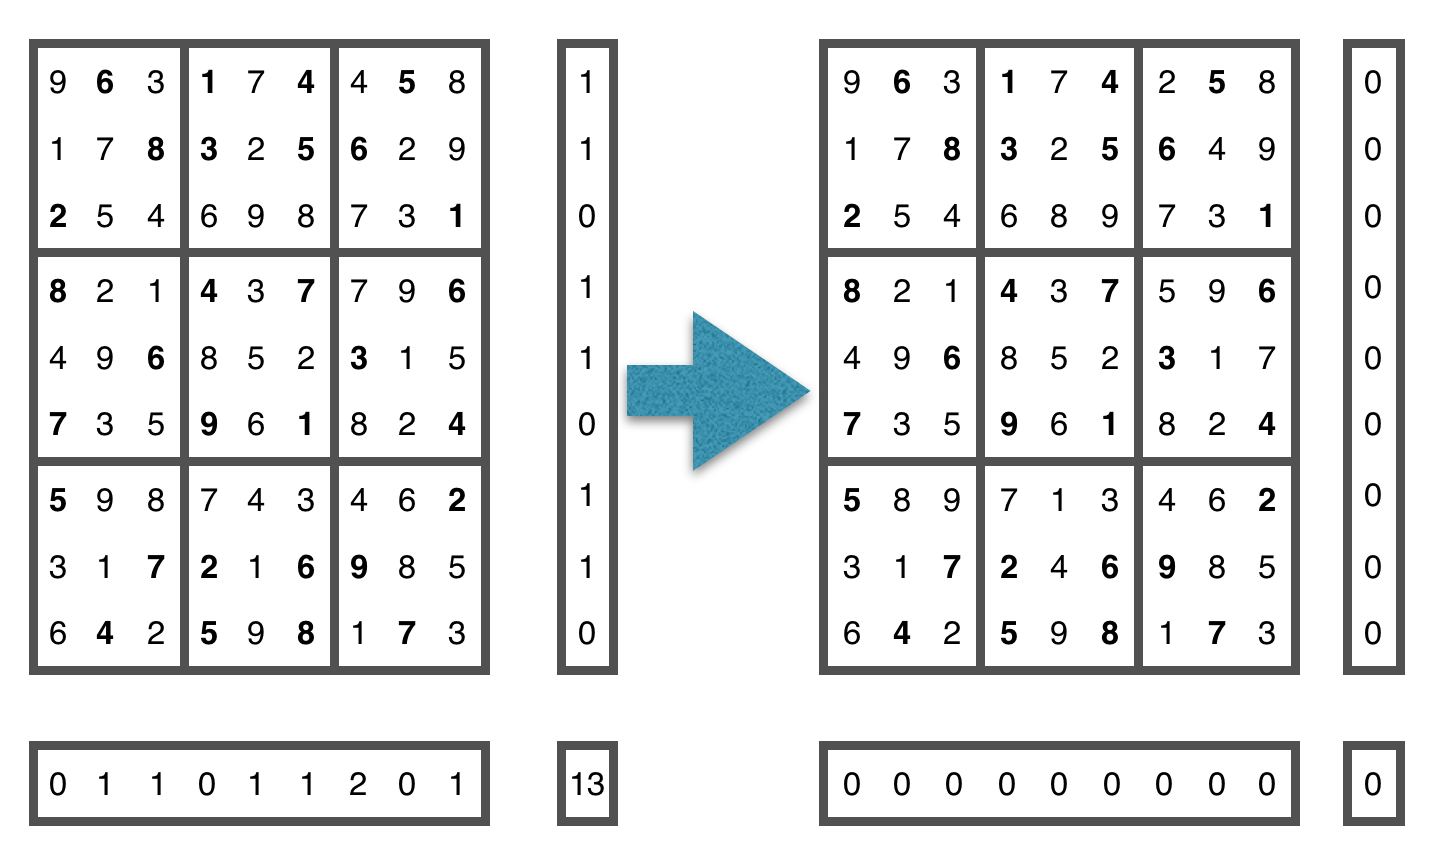
\includegraphics[scale=0.6]{imgs/costo.png}	
\paragraph{Solución vecina}
Partiendo de una posible solución parcial, se procede a generar una solución vecina diferente pero a su vez cercana. Para ello realizamos entre 1 y 9 cambios de celdas, elegidas de manera aleatoria, siempre intercambiando entre la misma caja para seguir asegurando la formulación (3), siempre y cuando las celdas no sean las iniciales o las correctas. Estos "pequeños" cambios, son parte de la búsqueda local, y como se verá más adelante, puede no ser descartada como camino a seguir.

\paragraph{Algoritmo}
\begin{algorithm}
\caption{Sudoku con Simulated annealing}\label{SimulatedAnnealing}
\begin{algorithmic}[1]
\Function{SASudokuSolver}{Inicio, $\alpha$, MaxIter, $Temp_{0}$ }

\State $sol_{0}$ $\gets$ generarSolucionInicial(inicio)
\State $solucionActual$  $\gets$ $mejorSudoku$   $\gets$ $sol_{0}$ 
\State $costoActual$ $\gets$ $mejorCosto$ $\gets$ costo(mejorSudoku)
\State \textbf{Mientras} no exceda las iteraciones m\'aximas y no haya encontrado una soluci\'on 

\State \indent  $nuevaSol$ $\gets$ busquedaLocal($solucionActual$)
\Comment{Se busca soluci\'on vecina}
\State \indent  $nuevoCosto$ $\gets$ costo($nuevaSol$)
\Comment {Se calcula el nuevo costo}
\State \indent  $aceptacion$ $\gets$ Rand(0,1) $<$ exp(($costoActual$ - $nuevoCosto$)/$temp$)
\Comment{Se calcula la aceptaci\'on, con un valor aleatorio entre (0,1)}
\State \indent\textbf{Si} se acepta como la soluci\'on actual y no fue usada antes
\State \indent\indent $solucionActual$ $\gets$ $nuevaSol$
\State \indent\indent $costoActual$ $\gets$ $nuevoCosto$
\State \indent\indent Marcar la soluci\'on como ya usada
\State \indent\textbf{Fin Si}
\State \indent\textbf{Si} el costo de la actual es menor que la mejor soluci\'on
\State \indent\indent $mejorSudoku$ $\gets$ $solucionActual$
\State \indent\indent $mejorCosto$ $\gets$ $costoActual$
\State \indent\indent $temp$ $\gets$ $Temp_{0}$
\Comment Reiniciamos la temperatura
\State \indent\textbf{Fin Si}
\State \indent\textbf{Si} el costo de la nueva soluci\'on vecina es 0
\State \indent\indent Devolver $nuevaSol$
\Comment Devolvemos esa soluci\'on del Sudoku
\State \indent\indent Finalizamos la funci\'on
\State \indent\textbf{Fin Si}
\State \indent $temp$ $\gets$ M\'aximo entre 0.1 y $\alpha$ * $temp$
\Comment Le aseguramos un piso mínimo a la temperatura
\State \textbf{Fin Mientras}
\State Devolver $mejorSudoku$
\Comment Devolvemos la mejor soluci\'on del Sudoku que hayamos encontrado
\EndFunction
\end{algorithmic}
\end{algorithm}

\begin{algorithm}
\caption{B\'usqueda local}\label{BusquedaLocal}
\begin{algorithmic}[1]
\Function{BusquedaLocal}{Solucion}
\State \textbf{Repetir} entre 1 y 9 veces
\State\indent $celdaAleatoria$ $\gets$ $seleccionarCeldaAleatoria(Solucion)$
\Comment Seleccionar una celda aleatoria
\State\indent $otraCelda$ $\gets$ $seleccionarOtraCeldaAleatoria(celdaAleatoria)$
\Comment Seleccionar otra celda aleatoria del mismo cuadrante
\State\indent \textbf{Si} ninguna de las dos celdas seleccionadas est\'a protegida
\State\indent\indent $Swap(Solucion, celdaAleatoria, otraCelda)$ 
\Comment Intercambiar celdas
\State\indent \textbf{Fin Si}
\State \textbf{Fin del ciclo}
\State Devolver soluci\'on vecina

\EndFunction
\end{algorithmic}
\end{algorithm}

\begin{algorithm}
\caption{Generar soluci\'on inicial}\label{GenerarSolucionInicial}
\begin{algorithmic}[1]
\Function{GenerarSolucionInicial}{SudokuInicial}
\State \textbf{Mientras haya cambios}
\State\indent \textbf{Por} cada celda del suduoku
\State\indent\indent Recorrer toda su fila y toda su columna recolectando los valores
\State\indent\indent Intersectar la recolecci\'on con los valores del 1 al 9
\Comment Para calcular los posibles valores de la fila
\State\indent\indent \textbf{Si s\'olo queda un posible valor}
\State\indent\indent \indent Asignarselo a la celda
\State\indent\indent \indent Proteger la celda
\State\indent\indent \indent Marcar que hubo cambio
\State\indent\indent \textbf{Fin Si}
\State\indent \textbf{Fin del ciclo} 
\State \textbf{Fin Mientras}
\State \textbf{Por} cada celda vacia
\State\indent Seleccionar uno de los posibles valores que puede tener la celda 
\State\indent En caso de que no tenga, elegir un valor aleatoria que falte en la misma caja que se encuentra la celda
\State \textbf{Fin del ciclo}
\EndFunction
\end{algorithmic}
\end{algorithm}

